\section{Анализ предметной области}

\begin{frame}
\frametitle{Варианты использования}
\begin{figure}
    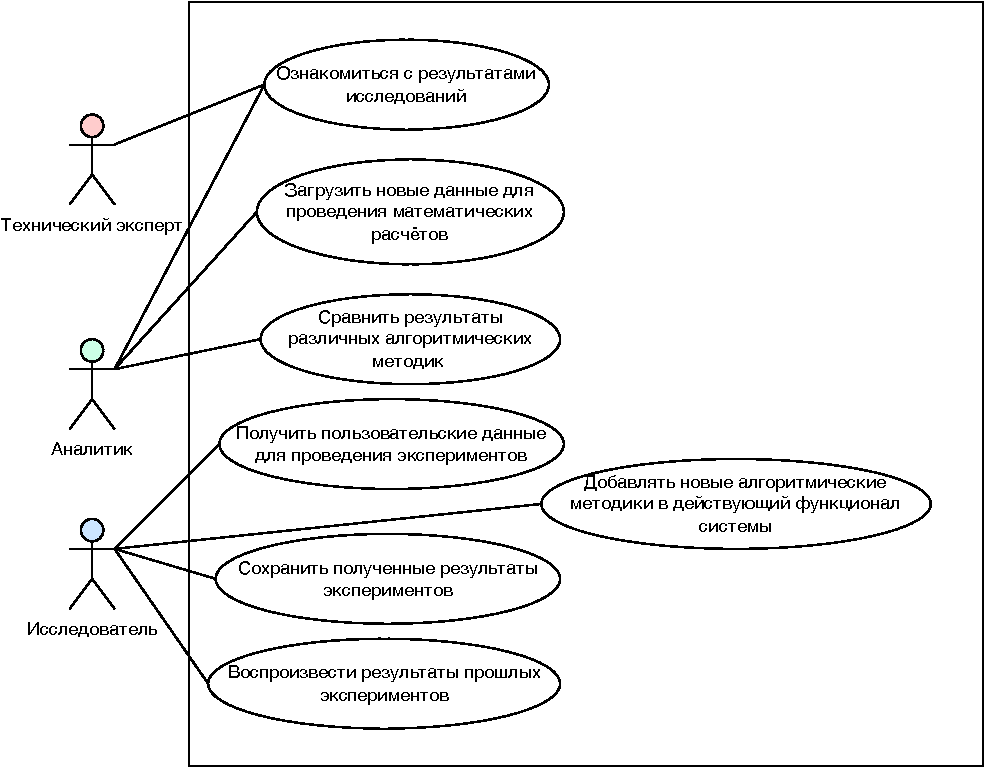
\includegraphics[scale=.48]{pictures/analysis/usecase}
    \caption{Диаграмма вариантов использования}
\end{figure}
\end{frame}

\begin{frame}
\frametitle{Бизнес-процессы}
\begin{figure}
    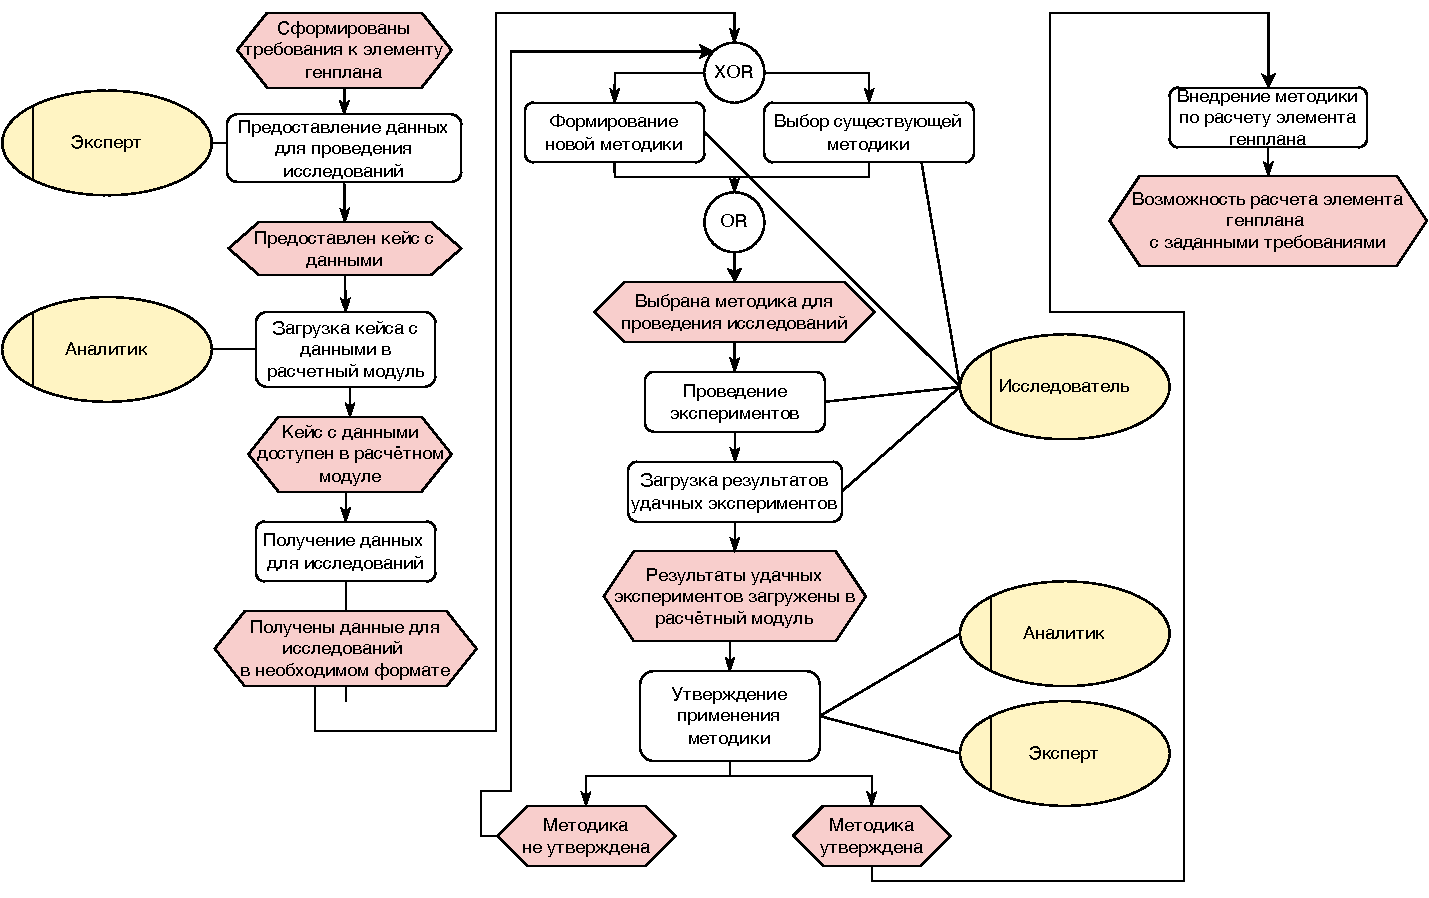
\includegraphics[scale=.48]{pictures/analysis/common_epc}
\end{figure}
\end{frame}

\begin{frame}
\frametitle{Бизнес-процессы}
\begin{figure}
    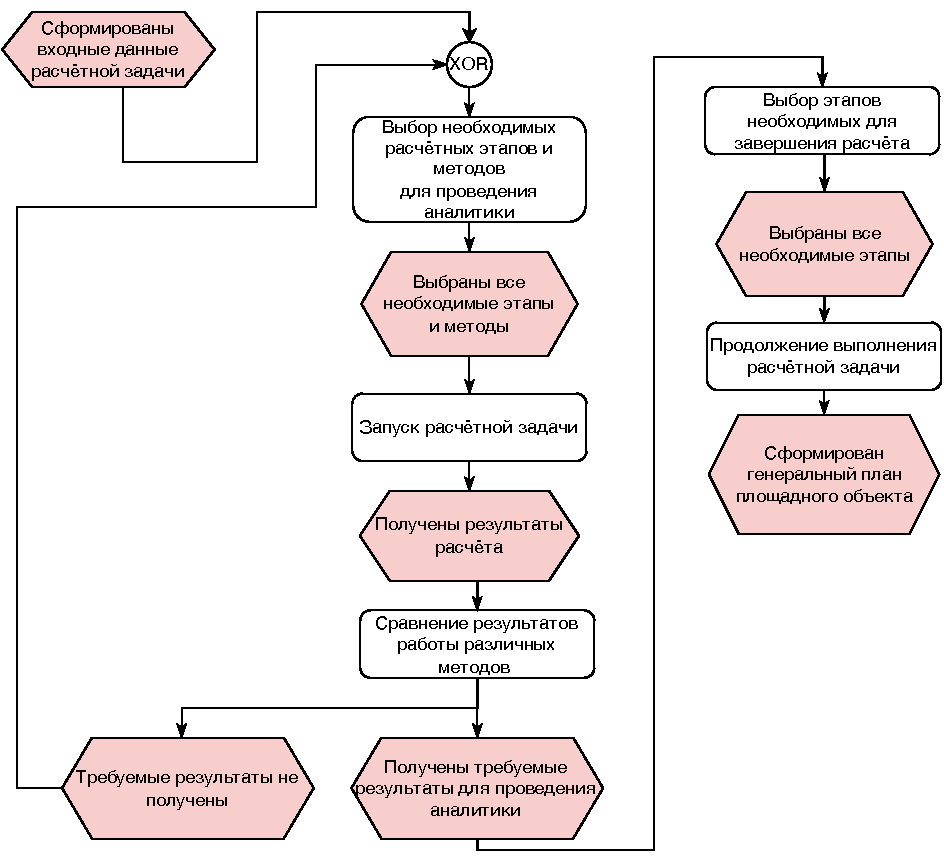
\includegraphics[scale=.49]{pictures/analysis/analytics_epc}
\end{figure}
\end{frame}


\begin{frame}
\frametitle{Предметная область задачи}
\begin{columns}[c]

\column{.45\textwidth}{
    Входные данные
    \begin{enumerate}
        \item допустимая для строительства область на карте;
        \item стоимостная модель расчета стоимости инженерной подготовки;
        \item перечень сооружений;
        \item параметры коммуникаций между сооружениями проектируемого объекта;
        \item параметры цифровой модели рельефа;
    \end{enumerate}
}

\column{.45\textwidth}{
    Выходные данные
    \begin{itemize}
        \item фигура площадного объекта;
        \item местоположения сооружений;
        \item схема технологических эстакад минимальной длины;
        \item схема внутриплощадочных проездов;
        \item стоимость инженерной подготовки;
        \item зоны распространения теплового потока;
        \item зоны распространения взрывной волны;
    \end{itemize}
}
\end{columns}
\end{frame}


\section{Формирование требований}

\begin{frame}
\frametitle{Функциональные требования}
\begin{itemize}
    \item {
        Возможность расчёта генерального плана площадного объекта в автоматическом режиме.
    }
    \item {
        Расчёт генплана должен представлять последовательность этапов.
    }
    \item {
        Результат каждого этапа расчёта должен быть сохранён в долговременное хранилище.
    }
    \item {
        Возможность продолжить расчёт с последнего успешно завершенного этапа.
    }
    \item {
        Возможность сравнения одинаковых расчётных объектов, полученных путем применения различных методик.
    }
    \item {
        Возможность загрузки данных, полученных от технических экспертов, в расчётный модуль.
    }
    \item {
        Возможность загрузки результатов экспериментов, а также информации об особенностях
        проведения экспериментов в расчётный модуль.
    }
\end{itemize}
\end{frame}


\begin{frame}
\frametitle{Нефункциональные требования}
\begin{itemize}
    \item {
        Проведение исследований на вычислительном сервере с операционной системой Ubuntu 20.04 LTS.
    }
    \item {
        Осуществление вызова алгоритмически сложной части системы в отдельном процессе.
    }
    \item {
        Разработанные алгоритмы должны быть оформлены в отдельную библиотеку, имеющей версионирование.
    }
    \item {
        Обеспечение высокой скорости добавления алгоритмических методик в проект.
    }
    \item {
        Обеспечение высокого уровня гибкости системы.
    }

\end{itemize}
\end{frame}